\documentclass{beamer}

\usetheme{CambridgeUS}

\usepackage{fourier}

\usefonttheme{professionalfonts} % using non standard fonts for beamer
\usefonttheme{serif} % default family is serif
\usepackage{fontspec}
\setmainfont{ClearSans-Regular.ttf}

\usepackage{tcolorbox}
\usepackage{lipsum}

\usepackage{algorithm}
\usepackage{algpseudocode}
\makeatletter
%\algrenewcommand\ALG@beginalgorithmic{\tiny}
\makeatother

% NEW COMMENTS
\newcommand{\MO}{\mathcal{O}}


% SECTION TITLE SLIDE

\AtBeginSection[]{
	\begin{frame}[plain]
	\vfill
	
	\centering
	\begin{beamercolorbox}[center,rounded=true]{body}
		\usebeamerfont{title}\insertsectionhead\par%
	\end{beamercolorbox}
	\rule{20pt}{1pt}
	\vfill
\end{frame}
}


% COLOR
\definecolor{C}{HTML}{20639b}
\definecolor{CL}{HTML}{FCB76F}
\definecolor{CD}{HTML}{541D61}
\definecolor{GrD}{HTML}{8F3066}
\definecolor{GrL}{HTML}{EEEEEE}

\definecolor{W}{HTML}{FFFFFF}

\setbeamercolor{palette primary}{fg = W,bg = CD}
\setbeamercolor{palette secondary}{fg = CL,bg = CD}
\setbeamercolor{palette tertiary}{fg = CL,bg = CD}
\setbeamercolor{palette quaternary}{fg = CL,bg = CD}

\setbeamercolor{title}{fg = CL,bg = CD}
\setbeamercolor{titlelike}{fg = CD,bg = W}

\setbeamertemplate{blocks}[rounded][shadow=false]
\setbeamercolor{block title}{bg=GrD, fg=W}
\setbeamercolor{block body}{bg=GrL}

\setbeamertemplate{itemize item}[circle]
\setbeamertemplate{itemize subitem}[circle]

\setbeamercolor{itemize item}{fg=CD}
\setbeamercolor{itemize subitem}{fg=CD}
\setbeamercovered{transparent}

% IMAGES
\usepackage{graphicx}

% MATH
\usepackage{amsthm,amsmath,amssymb}
\newtheorem{observation}{Observation}
\newtheorem{conjecture}{Conjecture}
\newtheorem{proposition}{Proposition}
\newtheorem{lem}{Lemma}
\newcommand{\R}{\Bbb{R}}
\newcommand{\E}{\Bbb{E}}
\newcommand{\D}{\mathcal{D}}
\newcommand{\Ll}{\mathcal{L}}
\newcommand{\BigO}{\mathcal{O}}

\title[IPC: Highly Communicative Processes]{\normalsize{Feasibility Study of Local IPC Mechanisms in Support of Highly Communicative Processes}}
\author[]{Amir Hossein Sorouri\\ \tiny{\href{mailto:amir_sorouri@iust.ac.ir}{amir\_sorouri@iust.ac.ir}}\\ \vspace{6pt} \small{Supervisor:}\\ \normalsize Professor Mohsen Sharifi\\}
\institute{Iran Univeristy of Science and Technology \\}
\titlegraphic{
	\includegraphics[width=2cm]{ut.png}
}

\begin{document}
	\maketitle
	\section{Recall From Inter-Process Communication Basics}
	
	\begin{frame}{IPC Models}
		\begin{columns}
			\begin{column}{0.65\textwidth}
				\begin{itemize}
					\vspace{4pt} \item <1-> A set of IPC Mechanisms;
					\begin{itemize}
						\vspace{4pt} \item <1-> File;
						\vspace{4pt} \item <1-> Signal;
						\vspace{4pt} \item <1-> Socket;
						\begin{itemize}
							\vspace{4pt} \item <1-> Unix
							\vspace{4pt} \item <1-> Others
						\end{itemize}
						\vspace{4pt} \item <1-> File Descriptor;
						\begin{itemize}
							\vspace{4pt} \item <1-> Named
							\vspace{4pt} \item <1-> Un-Named
						\end{itemize}
						\vspace{4pt} \item <1-> Shared Memory;
						\vspace{4pt} \item <1-> Message Passing;
						\vspace{4pt} \item <1-> Cross Memory Attach;			
					\end{itemize}
				\end{itemize}
			\end{column}
			\begin{column}{0.35\textwidth}
				\begin{figure}
					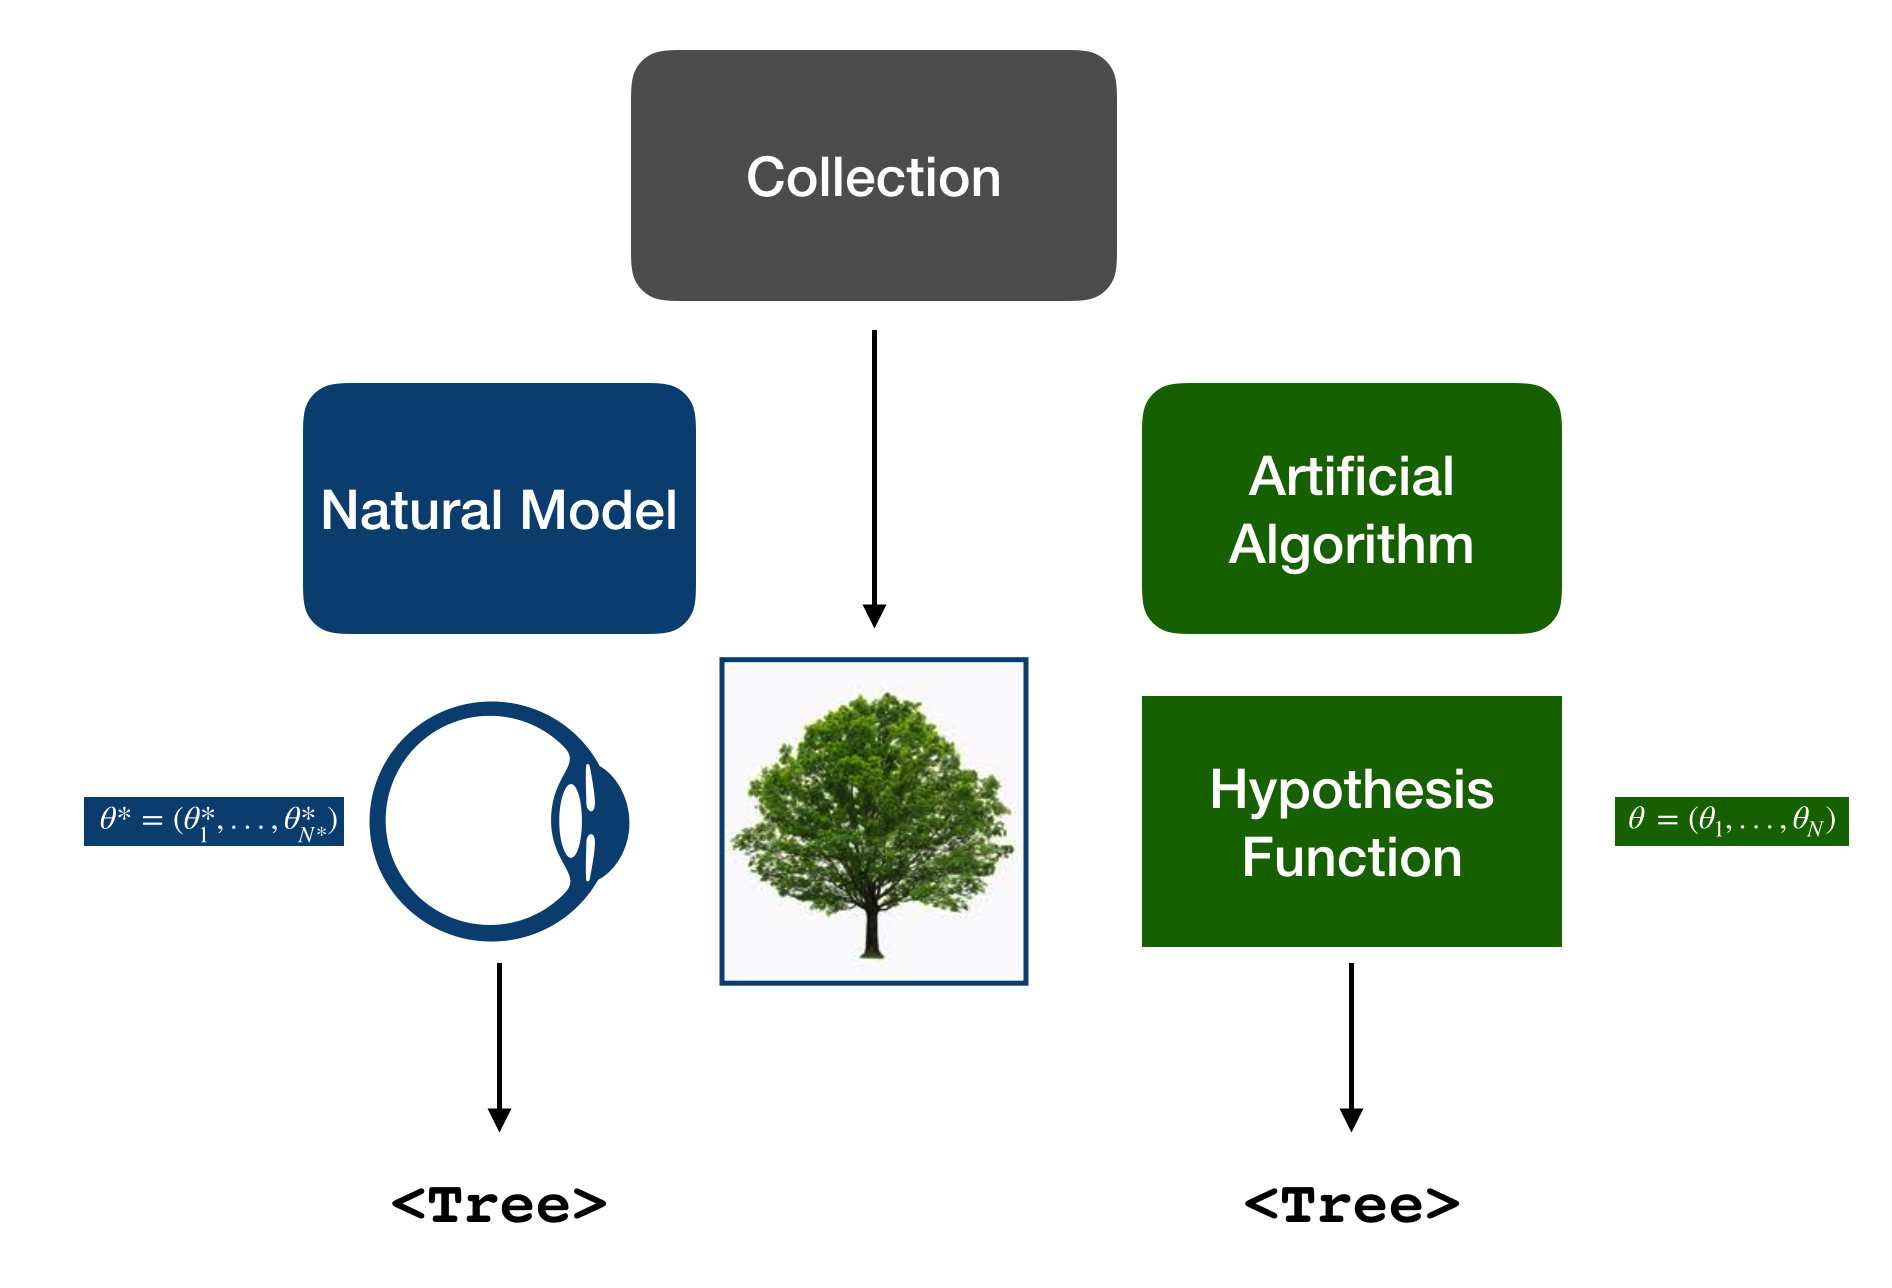
\includegraphics[width=0.8\textwidth,height=0.7\textwidth]{Pics/learning-algorithm.png}
				\end{figure}
				\begin{figure}
					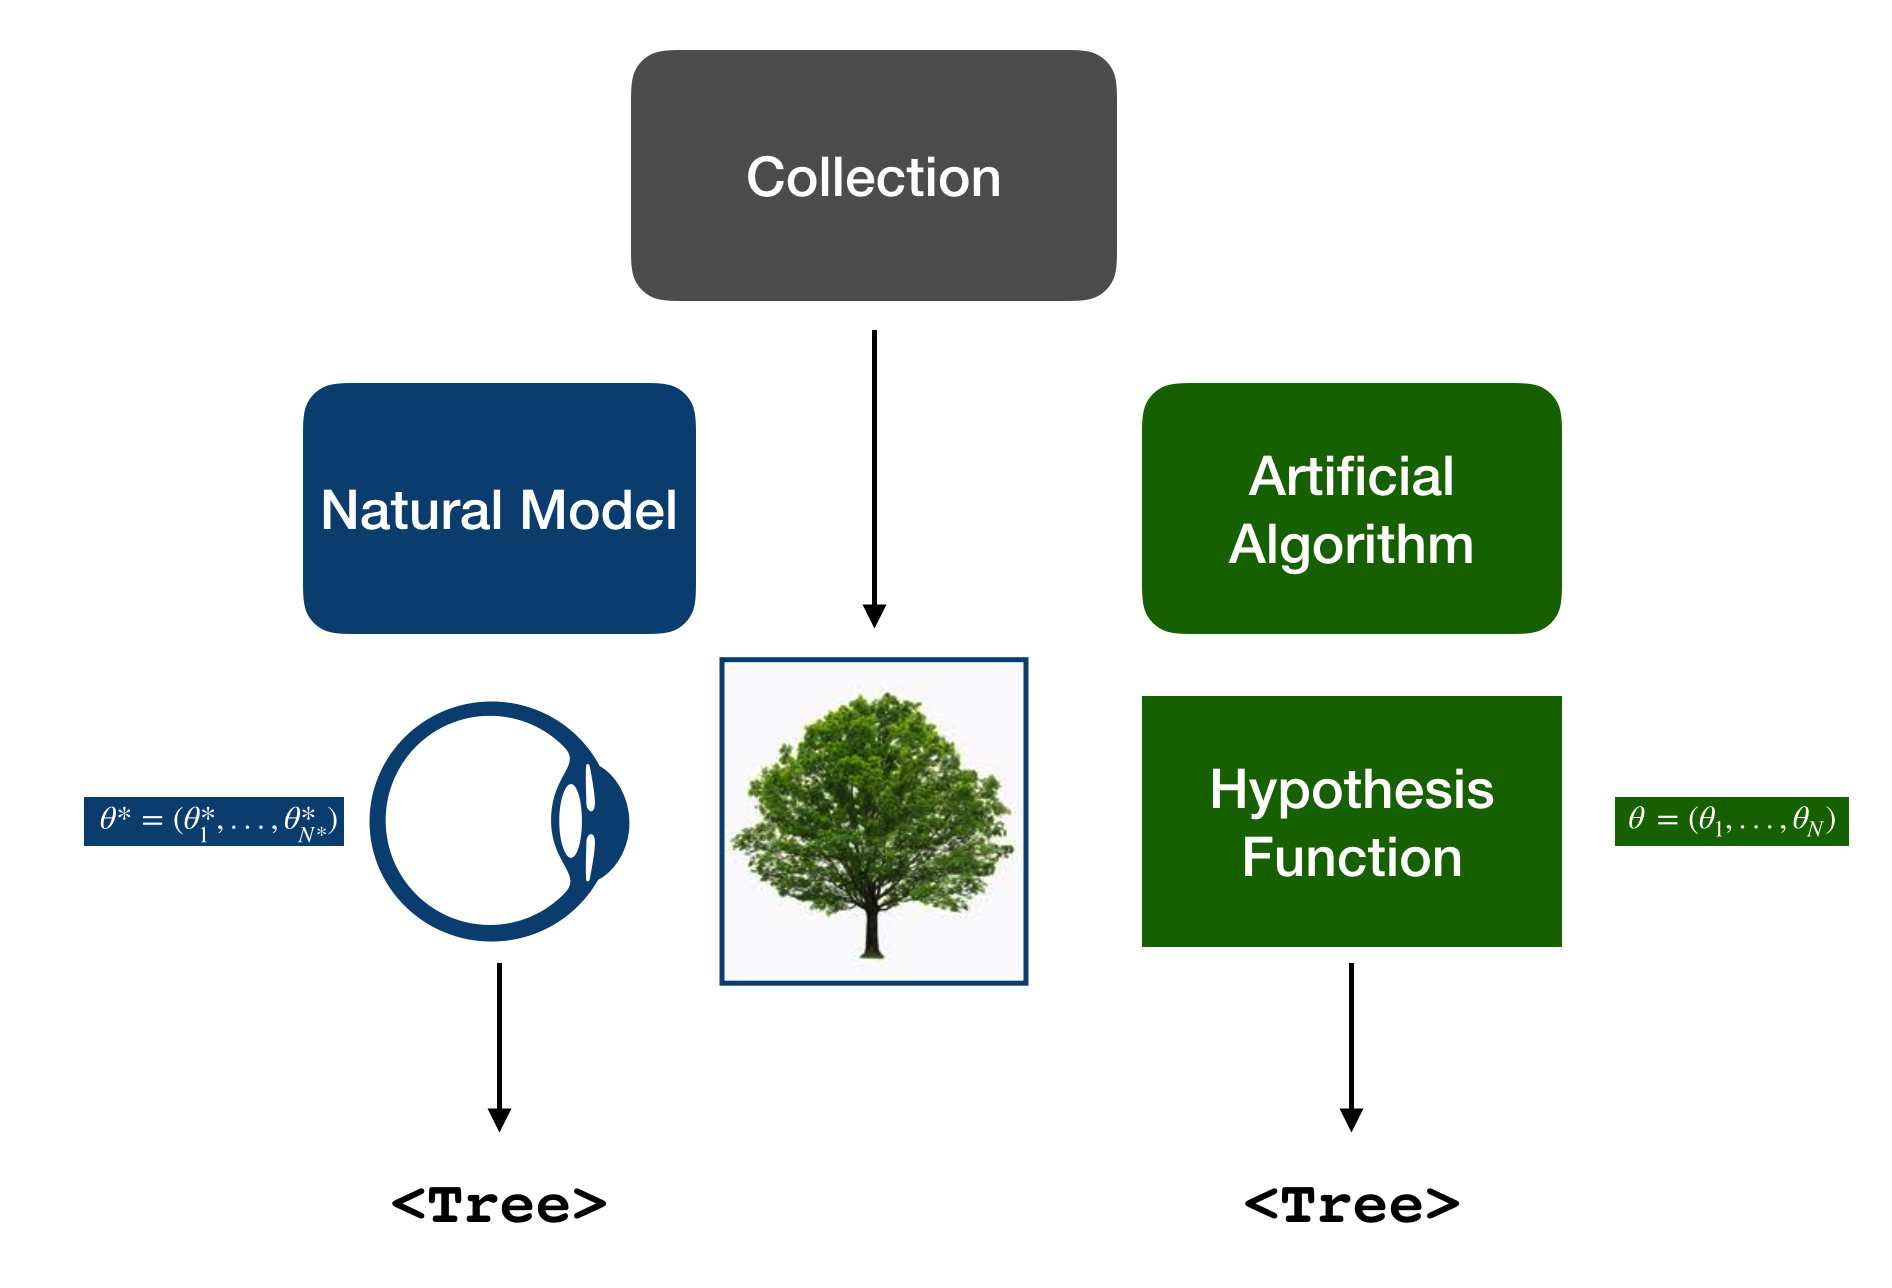
\includegraphics[width=0.8\textwidth,height=0.7\textwidth]{Pics/learning-algorithm.png}
				\end{figure}
			\end{column}
		\end{columns}
	
	\end{frame}

	\begin{frame}{Synchronization Models}
		\begin{itemize} 
			 \item There are \alert{Two} types/models of Synchronization
			\begin{itemize}
				\vspace{8pt} \item \alert{Blocking}
				\vspace{8pt} \item \alert{Busy-waiting}
				\begin{itemize}
					\vspace{8pt} \item Busy-waiting
					\vspace{8pt} \item Spin-lock
					\vspace{8pt} \item Polling
				\end{itemize}
				\vspace{8pt} \item { \alert{Non-}Blocking \& \alert{Non-}Busy-waiting}
				\begin{itemize}
					\vspace{8pt} \item Lock-free
					\vspace{8pt} \item Wait-free
					\vspace{8pt} \item Non-blocking
				\end{itemize}
			\end{itemize}
		\end{itemize}
	\end{frame}
	
	\section{High Performance Computing (HPC) Concerns}
	\begin{frame}{Workflow Computation Model}
		content...
	\end{frame}
	\begin{frame}{OS-Noise influence on HPC Applications performance}
		content...
	\end{frame}
	
	\section{Related Works in Terms of HPC}
	\begin{frame}{Related Works In HPC}
		\begin{itemize}
			\vspace{8pt} \item \alert{Argo}
			\vspace{8pt} \item \alert{FFMK}
			\begin{itemize}
				\vspace{8pt} \item XEMEM
				\vspace{8pt} \item Kitten
				\vspace{8pt} \item Palacios
			\end{itemize}
			\vspace{8pt} \item \alert{Netmap}
			\begin{itemize}
				\vspace{8pt} \item Berkeley Packet Filter
				\vspace{8pt} \item DPDK
			\end{itemize}
		\end{itemize}
	\end{frame}
	
	\section{Related Works in Terms of IPC}
	\section{Evaluation}
	\section{Future Works}
	content...
\end{document}


